\documentclass[13pt,a4paper]{report}
\usepackage[margin=0.6in]{geometry}
\usepackage{fancybox}
\usepackage[utf8]{inputenc}
\usepackage[vietnamese,main=english]{babel}
\usepackage{multicol}
\usepackage{tabularx}
\usepackage{lmodern}
\usepackage{indentfirst}
\usepackage{float}
\usepackage{enumitem}
\usepackage{afterpage}
\usepackage[super]{nth}
\usepackage{titlesec}
\usepackage{bigdelim}
\usepackage[titles]{tocloft}
\usepackage{makecell}
\usepackage{arydshln}
\usepackage{perpage} %the perpage package
\usepackage{graphicx}
\usepackage{caption}
\usepackage{minted}
\usepackage{gensymb}
\usepackage{tikz}
\usepackage{circuitikz}
\usepackage{pgfplots}
\usepackage{cancel}
\usepackage{xurl}
\usepackage[bottom]{footmisc}
\usepackage[font=footnotesize,labelfont={scriptsize}]{subfig}
\usepackage{wrapfig}
\usepackage{latexsym,amssymb,amsmath}
%\usepackage{algpseudocode}
\usepackage{tocvsec2}
\usepackage{fancyref}
\usepackage{bookmark}
\usepackage{hyperref}
\usepackage[nameinlink,noabbrev]{cleveref}

\newcolumntype{Y}{>{\centering\arraybackslash}X}

\PassOptionsToPackage{hyphens}{url}

\makeatletter
\pgfcircdeclarebipole{}{\ctikzvalof{bipoles/vsourceam/height}}{vsourceAM}{\ctikzvalof{bipoles/vsourceam/height}}{\ctikzvalof{bipoles/vsourceam/width}}{%
  \pgfsetlinewidth{\pgfkeysvalueof{/tikz/circuitikz/bipoles/thickness}\pgfstartlinewidth}
   \pgfpathellipse{\pgfpointorigin}{\pgfpoint{0}{\pgf@circ@res@up}}{\pgfpoint{\pgf@circ@res@left}{0}}
   \pgfusepath{draw}
   \pgfscope
       \pgftransformxshift{0.6*\ctikzvalof{bipoles/vsourceam/margin}\pgf@circ@res@left}
       \pgftext[rotate=-\pgf@circ@direction]{$+$}
       \pgfusepath{draw}
   \endpgfscope
   \pgfscope
       \pgftransformxshift{0.6*\ctikzvalof{bipoles/vsourceam/margin}\pgf@circ@res@right}
       \pgftext[rotate=-\pgf@circ@direction]{$-$}
       \pgfusepath{draw}
   \endpgfscope
}
\makeatother

\MakePerPage{footnote} %the perpage package command
\usetikzlibrary{shapes,positioning,arrows,calc,automata}

\newcommand*\justify{%
  \fontdimen2\font=0.4em% interword space
  \fontdimen3\font=0.2em% interword stretch
  \fontdimen4\font=0.1em% interword shrink
  \fontdimen7\font=0.1em% extra space
  \hyphenchar\font=`\-% allowing hyphenation
}
\renewcommand\cftchapafterpnum{\vskip-2pt}
\renewcommand\cftsecafterpnum{\vskip-2pt}

\renewcommand{\theequation}{\arabic{equation}}

% FLOW CHART
\tikzstyle{startstop} = [rectangle, rounded corners, minimum width=3cm, minimum height=1cm,text centered, draw=black, fill=red!30]
\tikzstyle{io} = [trapezium, trapezium left angle=70, trapezium right angle=110, minimum width=3cm, minimum height=1cm, text centered, draw=black, fill=blue!30]
\tikzstyle{process} = [rectangle, minimum width=3cm, minimum height=1cm, text centered, draw=black, fill=orange!30, text width=4cm]
\tikzstyle{decision} = [diamond, aspect=2.5, minimum width=3cm, minimum height=1cm, text centered, draw=black, fill=green!30]
\tikzstyle{arrow} = [thick,->,>=stealth]

% CHAPTER FORMAT
\titleformat{\chapter}%[display]
{\bfseries\fontsize{25}{30}\selectfont\raggedright}% Format and size of title text
{\llap{%
    \rule[-6pt]{6cm}{1.18cm}\rule{6pt}{0pt}}% Black box to the left, lowered 6pt. The end rule is a horisontal space.
  \llap{% Number also to the left, on top of the black box.
    \fontsize{22}{44}\selectfont\color{white}\thechapter\rule{10pt}{0pt}}}{0pt}{}{}

\counterwithin{figure}{section}
\renewcommand{\thefigure}{\arabic{chapter}.\arabic{section}.\alph{figure}}

\renewcommand{\thetable}{\arabic{table}}

\renewcommand\labelitemi{$-$}
  
\titleformat{\section}
  {\LARGE\bfseries}{}{}{}
\renewcommand\thesection{\arabic{section}.}
\renewcommand\thesubsection{\arabic{subsection}}
\makeatletter
\renewcommand*\l@section{\@dottedtocline{1}{1.5cm}{2em}}
\renewcommand\section{\@startsection {section}{1}{-1em}%
  {-3.5ex \@plus -1ex \@minus -.2ex}%
  {2.3ex \@plus.2ex}%
  {\normalfont\Large\bfseries}}
\def\sectionmark#1{%
      \markright {\MakeUppercase{#1}}}
\makeatother

\titleformat{\subsection}
  {\normalfont\bfseries}{\thesubsection.}{0.5em}{}
\renewcommand\cftsubsecaftersnum{.} 
\renewcommand\thesubsection{\alph{subsection}}

\addto{\captionsenglish}{%
  \renewcommand{\bibname}{References}
}

%\addtocontents{toc}{\setcounter{tocdepth}{2}}
%\addtocontents{lof}{\vskip -1.6cm}
%\addtocontents{lot}{\vskip -1.6cm}

    
% TOC settings
\renewcommand\cftchapnumwidth{2.8em}
\renewcommand\cftsecnumwidth{3em}
\renewcommand\cftsecindent{3em}
\renewcommand\cftsubsecindent{5em}
\renewcommand\thechapter{\Roman{chapter}}
    
%\titleformat{\chapter}[display]{\normalfont\huge\bfseries}{}{0pt}{\Huge}
\newcommand{\hsp}{\hspace{20pt}}
%\titleformat{\chapter}[hang]{\Huge\bfseries}{\thechapter\hsp\textcolor{gray75}{|}\hsp}{0pt}{\Huge\bfseries}
\titleformat*{\subsubsection}{\large\bfseries}
%\titlespacing*{\chapter}{0pt}{0pt}{0pt}
    
\newcolumntype{P}[1]{>{\centering\arraybackslash}p{#1}}
\newcolumntype{C}{>{\centering\arraybackslash}p{4em}}
    
\setlist[itemize]{noitemsep, topsep=0pt}
%\AtBeginEnvironment{multicols}{\RaggedRight}

\titlespacing*{\chapter}{0pt}{0pt}{20pt}

\newcommand\Chapter[2]{\chapter
  [#1\text{: }\hfil\hbox{}\protect\linebreak{\itshape#2}]%
  {#1\\[-0.75ex]\Large#2}%
  \markboth{\MakeUppercase{\chaptername\ \thechapter.\ #1}}{}%
}


\def\doubleoverline#1{\overline{\overline{#1}}}

\captionsetup[subfloat]{labelformat=empty}

\begin{document}
%Trang bìa 1
\fontsize{13pt}{18pt}\selectfont
\begin{titlepage}
\thispagestyle{empty}
\thisfancypage{%đóng khung trang này
\setlength{\fboxsep}{0pt}% 8pt là độ dày của đường viền
\fbox}{} % phần nội dung sau là tương tự như đã làm
\

\begin{center}
\begin{large}
HO CHI MINH CITY UNIVERSITY OF TECHNOLOGY $-$ VNU HCMC
\end{large} \\
\begin{large}
OFFICE FOR INTERNATIONAL STUDY PROGRAM
\end{large} \\
\begin{large}
FACULTY OF ELECTRICAL AND ELECTRONIC ENGINEERING
\end{large} \\
\textbf{--------------------  *  --------------------}\\[4cm]
\includegraphics[scale=0.1]{logobk.png}\\[1cm]
{\fontsize{20pt}{1}\selectfont DIGITAL SYSTEMS (LAB)}\\
{\fontsize{20pt}{1}\selectfont EXPERIMENTAL REPORT (Lab 4)}\\[2.5cm]
\end{center}

\begin{otherlanguage}{vietnamese}
\begin{tabbing}
	\hspace{3.5cm}Lecturer  \ \ \ \ \=: \textbf{\parbox[t]{9cm}{Mr. Nguyễn Tuấn Hùng}}\\
	\hspace{3.5cm}Subject \>: \textbf{\parbox[t]{12cm}{Digital Systems}}\\
	\hspace{3.5cm}Class \>: \textbf{\parbox[t]{9cm}{TT06}}\\
	\hspace{3.5cm}Name \>: \textbf{\parbox[t]{9cm}{
		Lương Triển Thắng}}\\
	\hspace{3.5cm}Student ID \>: \textbf{\parbox[t]{9cm}{
		2051194}}\\[40pt]
\end{tabbing}
\end{otherlanguage}

\vspace{2.25cm}
\begin{center}
{\fontsize{13pt}{1}\selectfont Ho Chi Minh City, \nth{14} June, 2022}
\end{center}
\end{titlepage}

\tableofcontents

\setminted{fontsize=\normalsize}

\setcounter{chapter}{3}

\Chapter{Laboratory 4}{Finite State Machines}

\section{Know how to implement a FSM circuit and download the cicuit into the FPGA chip}
\subsection{Code}
\subsubsection{DFFn.vhd}
\begin{minted}{vhdl}
LIBRARY ieee;
USE ieee.std_logic_1164.ALL;
ENTITY DFFn IS
	PORT (
		Din, DClk, Dprs, Dclr, Den : IN STD_LOGIC;
		DQ : OUT STD_LOGIC);
END DFFn;
ARCHITECTURE Behavior OF DFFn IS
BEGIN
	PROCESS (Dprs, Dclr, DClk)
	BEGIN
		IF Dclr = '1' AND Dprs = '0' THEN
			DQ <= '0';
		ELSIF Dclr = '0' AND Dprs = '1' THEN
			DQ <= '1';
		ELSE
			IF rising_edge(DClk) AND Den = '1' THEN
				DQ <= Din;
			END IF;
		END IF;
	END PROCESS;
END Behavior;
\end{minted}

\subsubsection{NineDFF.vhd}
\begin{minted}{vhdl}
LIBRARY ieee;
USE ieee.std_logic_1164.ALL;
USE ieee.numeric_std.ALL;

ENTITY NineDFF IS
	PORT (
		NClk, Nen : IN STD_LOGIC;
		ND, Nprs, Nclr : IN STD_LOGIC_VECTOR(8 DOWNTO 0);
		NQ : OUT STD_LOGIC_VECTOR(8 DOWNTO 0)
	);
END NineDFF;

ARCHITECTURE arch OF NineDFF IS
	COMPONENT DFFn IS
		PORT (
			Din, DClk, Dprs, Dclr, Den : IN STD_LOGIC;
			DQ : OUT STD_LOGIC);
	END COMPONENT;
BEGIN
	gen : FOR i IN 8 DOWNTO 0 GENERATE
		DFFs : DFFn PORT MAP(
			Din => ND(i), DClk => NClk, Dprs => Nprs(i),
			Dclr => Nclr(i), Den => Nen, DQ => NQ(i));
	END GENERATE;
END ARCHITECTURE;
\end{minted}

\subsubsection{Exc1.vhd}
\begin{minted}{vhdl}
LIBRARY ieee;
USE ieee.std_logic_1164.ALL;
USE ieee.numeric_std.ALL;

ENTITY Exc1 IS
	PORT (
		clk, w, rstN : IN STD_LOGIC;
		LED : OUT STD_LOGIC_VECTOR(8 DOWNTO 0);
		z : OUT STD_LOGIC
	);
END Exc1;

ARCHITECTURE arch OF Exc1 IS
	SIGNAL D, Q, prsV, clrV : STD_LOGIC_VECTOR(8 DOWNTO 0);
	SIGNAL rst : STD_LOGIC;
	COMPONENT NineDFF IS
		PORT (
			NClk, Nen : IN STD_LOGIC;
			ND, Nprs, Nclr : IN STD_LOGIC_VECTOR(8 DOWNTO 0);
			NQ : OUT STD_LOGIC_VECTOR(8 DOWNTO 0)
		);
	END COMPONENT;
BEGIN
	rst <= NOT(rstN);

	D(8) <= w AND (Q(7) OR Q(8));
	D(7) <= Q(6) AND w;
	D(6) <= Q(5) AND w;
	D(5) <= w AND NOT(Q(5) OR Q(6) OR Q(7) OR Q(8));
	D(4) <= NOT(w) AND (Q(3) OR Q(4));
	D(3) <= Q(2) AND NOT(w);
	D(2) <= Q(1) AND NOT(w);
	D(1) <= NOT(Q(1) OR Q(2) OR Q(3) OR Q(4) OR w);
	D(0) <= '0';
	z <= Q(4) OR Q(8);

	-- FOR MODIFIED ONE-HOT
	--	D(8) <= w AND (Q(7) OR Q(8));
	--	D(7) <= Q(6) AND w;
	--	D(6) <= Q(5) AND w;
	--	D(5) <= w AND (NOT(Q(5) OR Q(6) OR Q(7) OR Q(8)));
	--	D(4) <= NOT(w) AND (Q(3) OR Q(4));
	--	D(3) <= Q(2) AND NOT(w);
	--	D(2) <= Q(1) AND NOT(w);
	--	D(1) <= NOT(Q(1) OR Q(2) OR Q(3) OR Q(4) OR w);
	--	D(0) <= '1';
	--	z <= Q(4) OR Q(8);

	LED <= Q;

	prsV <= "000000001" WHEN rst = '1' ELSE "000000000";
	clrV <= "111111110" WHEN rst = '1' ELSE "000000000";

	-- FOR MODIFIED ONE-HOT
	--	prsV <= "000000000" WHEN rst = '1' ELSE "000000000";
	--	clrV <= "111111111" WHEN rst = '1' ELSE "000000000";

	NDFF : NineDFF PORT MAP(
		NClk => clk, Nprs => prsV, Nclr => clrV,
		Nen => '1', ND => D, NQ => Q
	);
END ARCHITECTURE;
\end{minted}

\subsection{Waveform}
\subsubsection{One-hot}
\begin{figure}[H]
\centering
\includegraphics[scale=0.45]{images/Exc1_waveform_1.png}
\includegraphics[scale=0.45]{images/Exc1_waveform_2.png}
\end{figure}

\subsubsection{Modified one-hot}
\begin{figure}[H]
\centering
\includegraphics[scale=0.45]{images/Exc1_waveform_3.png}
\includegraphics[scale=0.45]{images/Exc1_waveform_4.png}
\end{figure}

\subsection{Result of RTL viewer}
\begin{figure}[H]
\centering
\subfloat[][D flip-flop]{
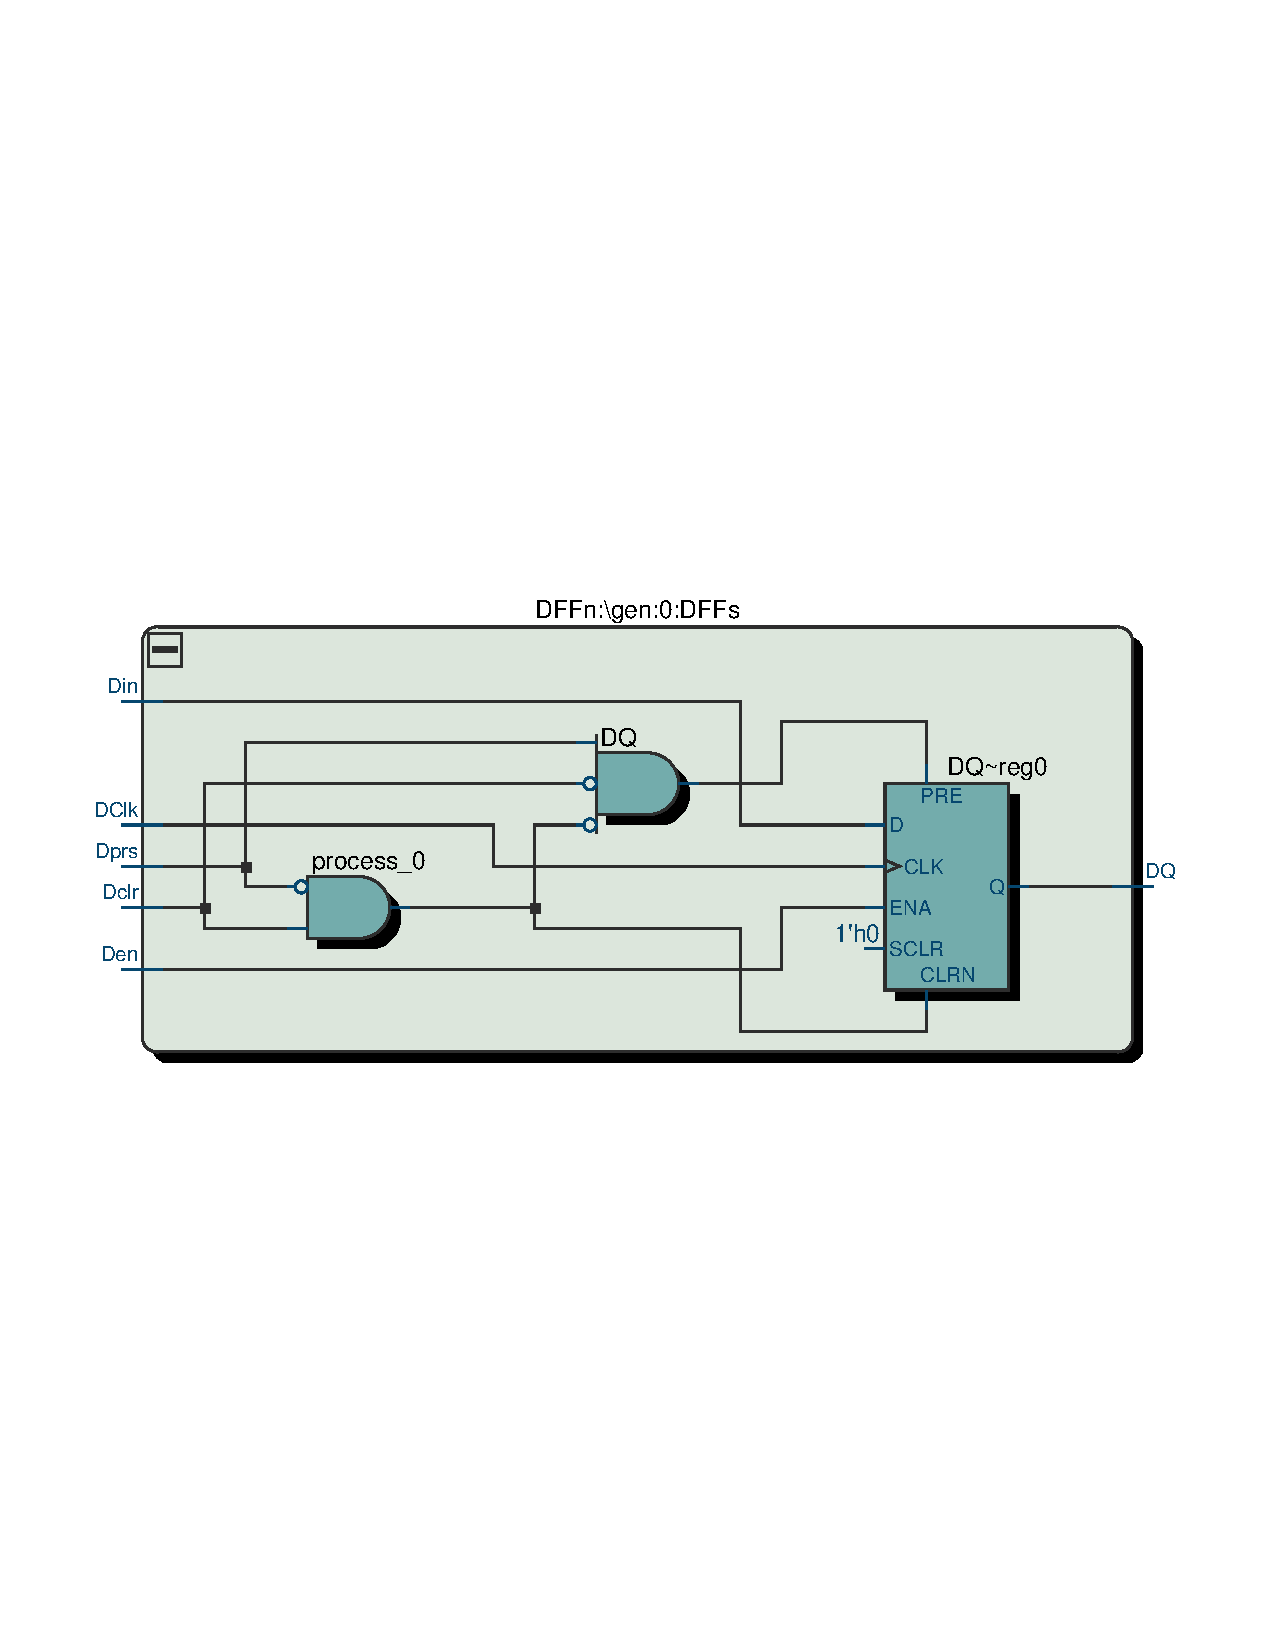
\includegraphics[scale=0.5, clip, trim={0cm 10cm 0cm 10.6cm}]{images/Exc1_DFF_RTL.pdf}
}
\subfloat[][Connected 9 D flip-flops]{
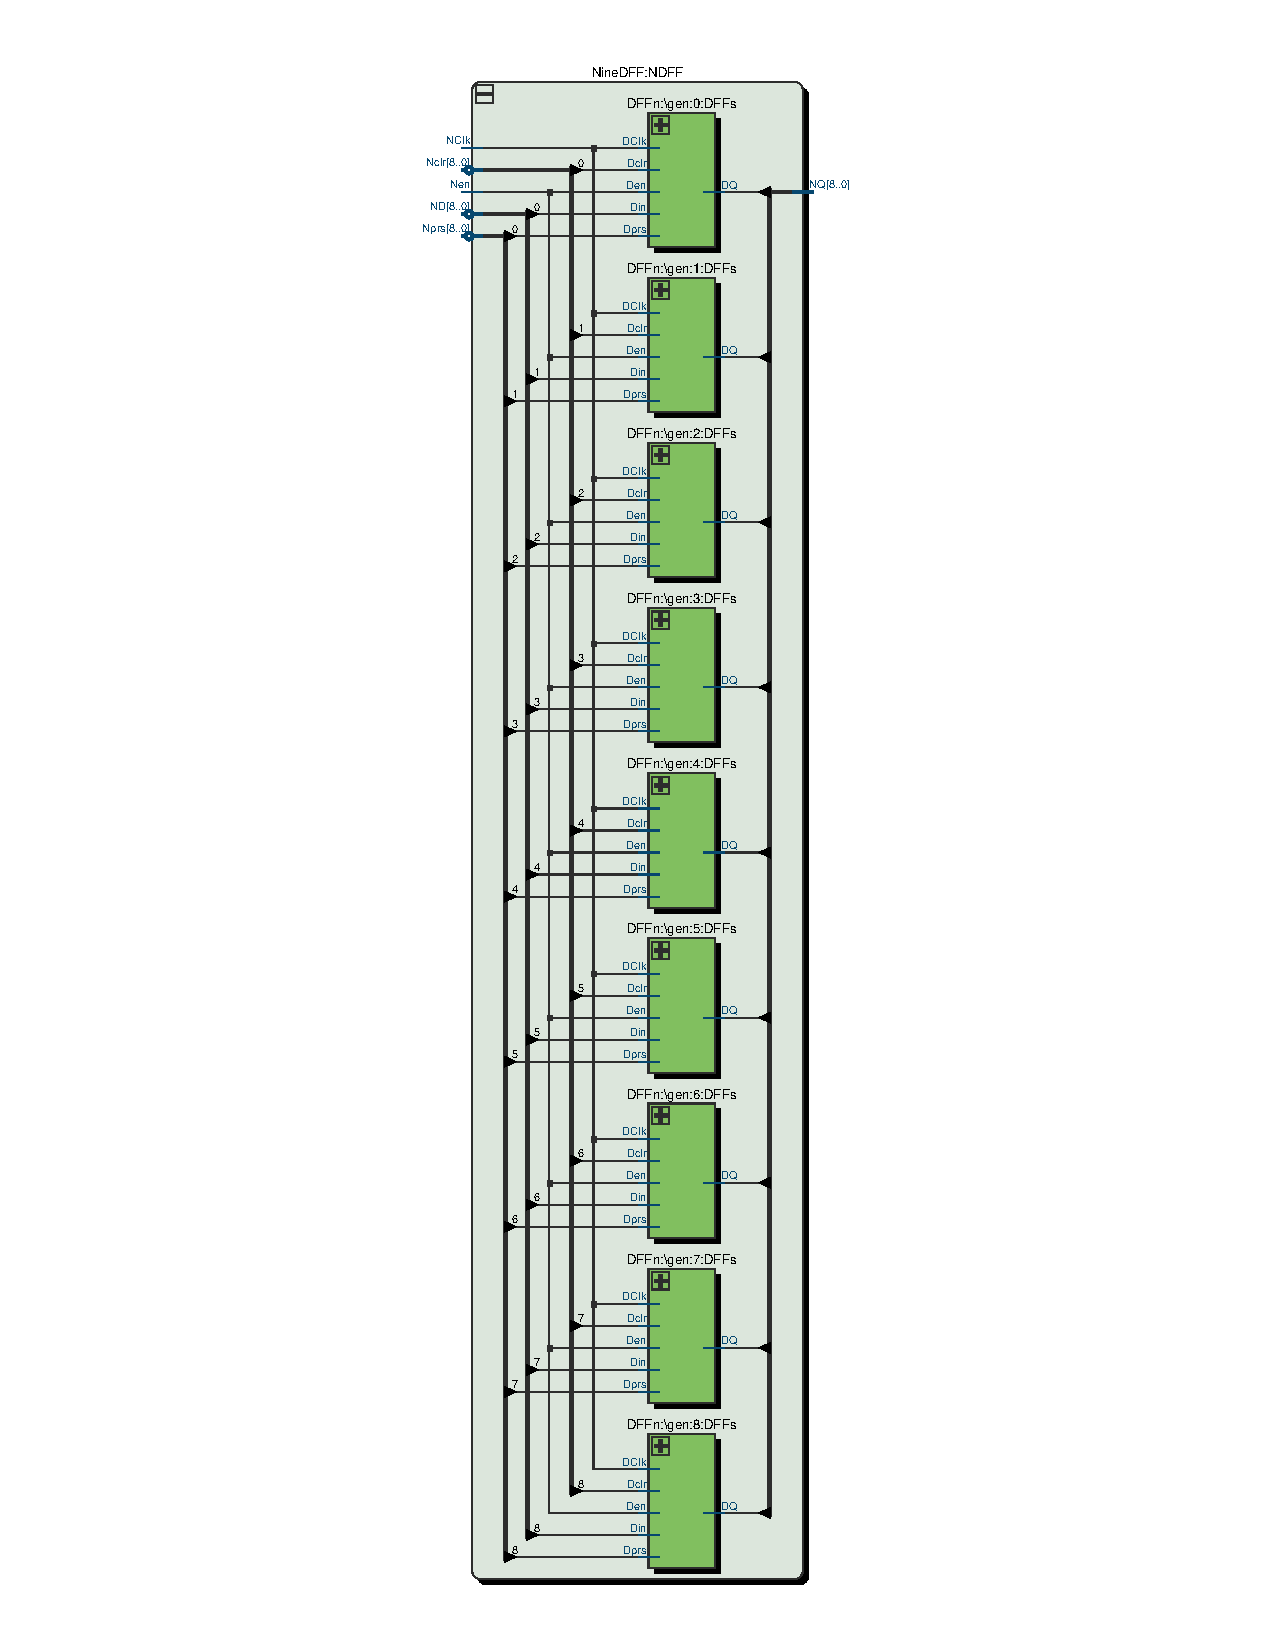
\includegraphics[scale=0.35, clip, trim={6cm 1cm 6cm 1.4cm}]{images/Exc1_NineDFF_RTL.pdf}
}
\end{figure}

\begin{figure}[H]
\centering
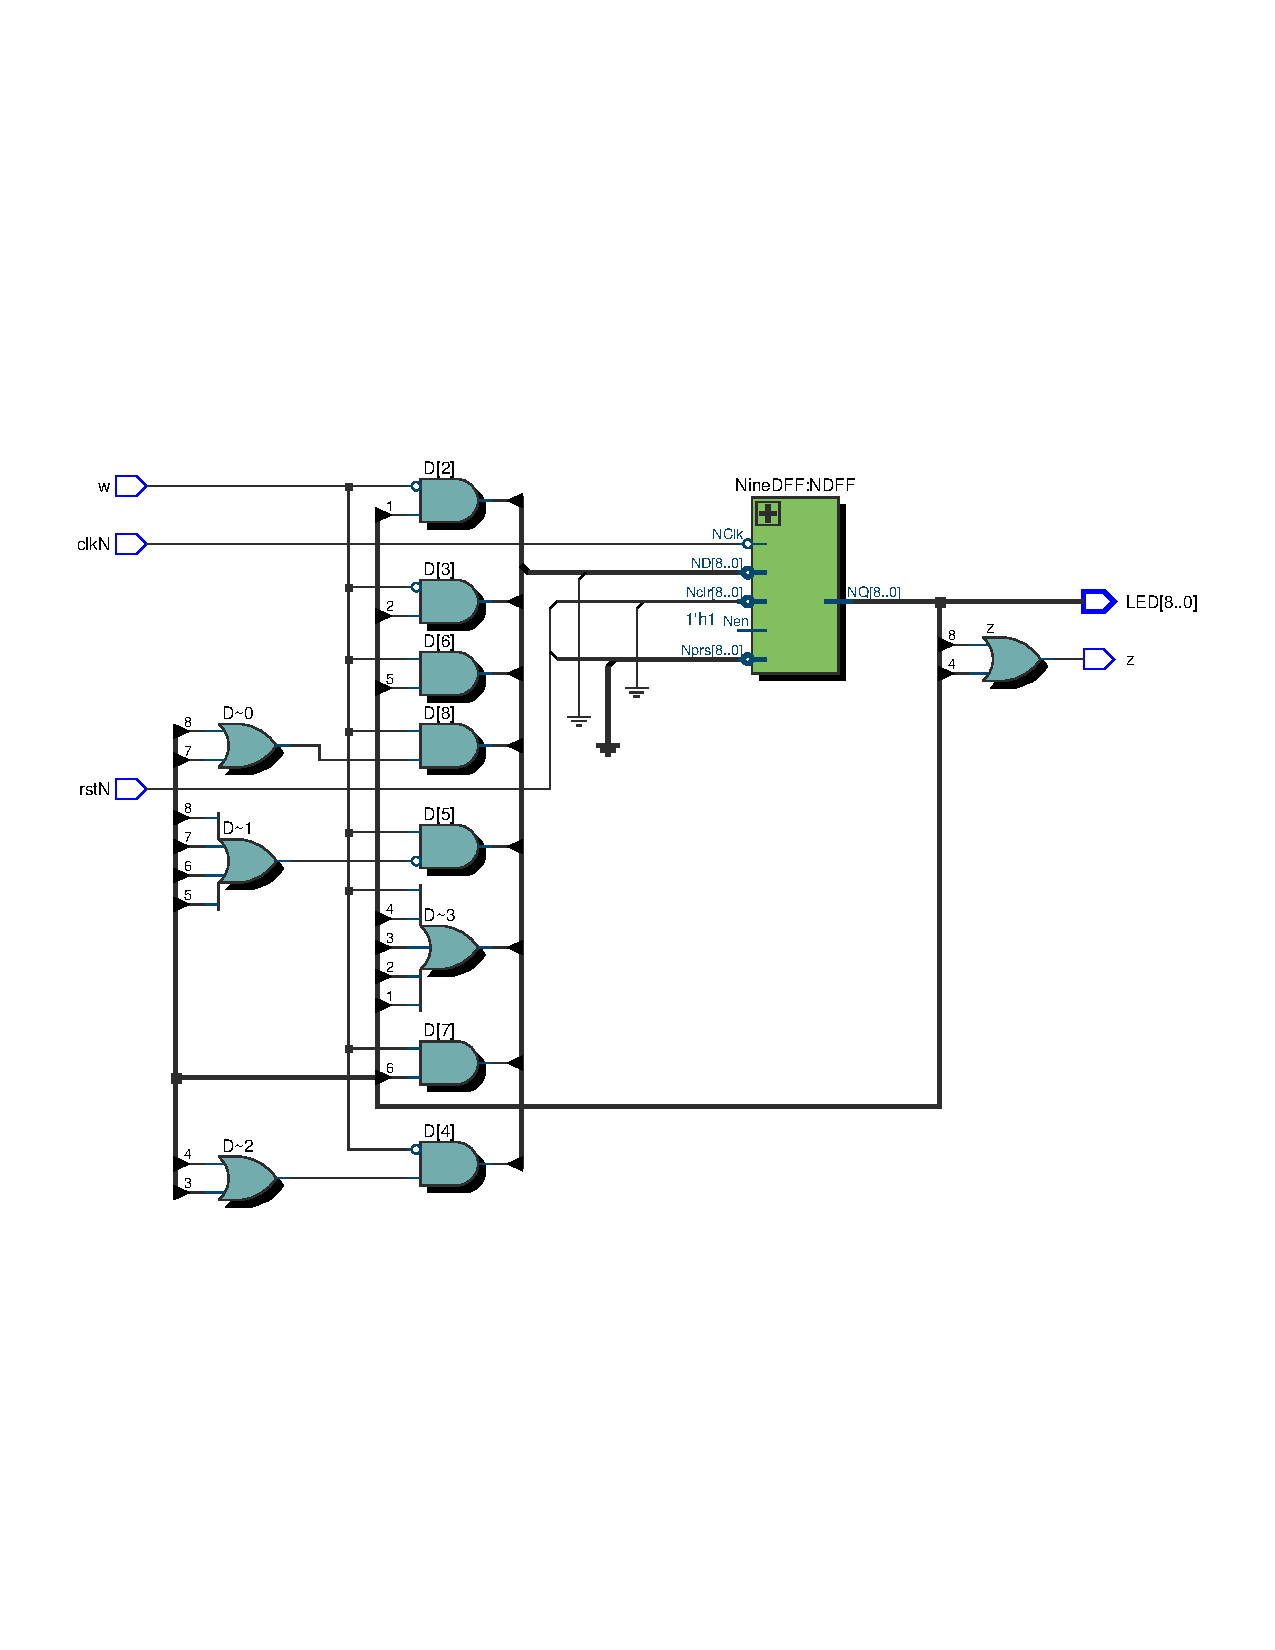
\includegraphics[scale=0.75, clip, trim={0cm 7.5cm 0cm 7.5cm}]{images/Exc1_RTL.pdf}
\caption*{Top level (using one-hot encoding)}
\end{figure}

\begin{figure}[H]
\centering
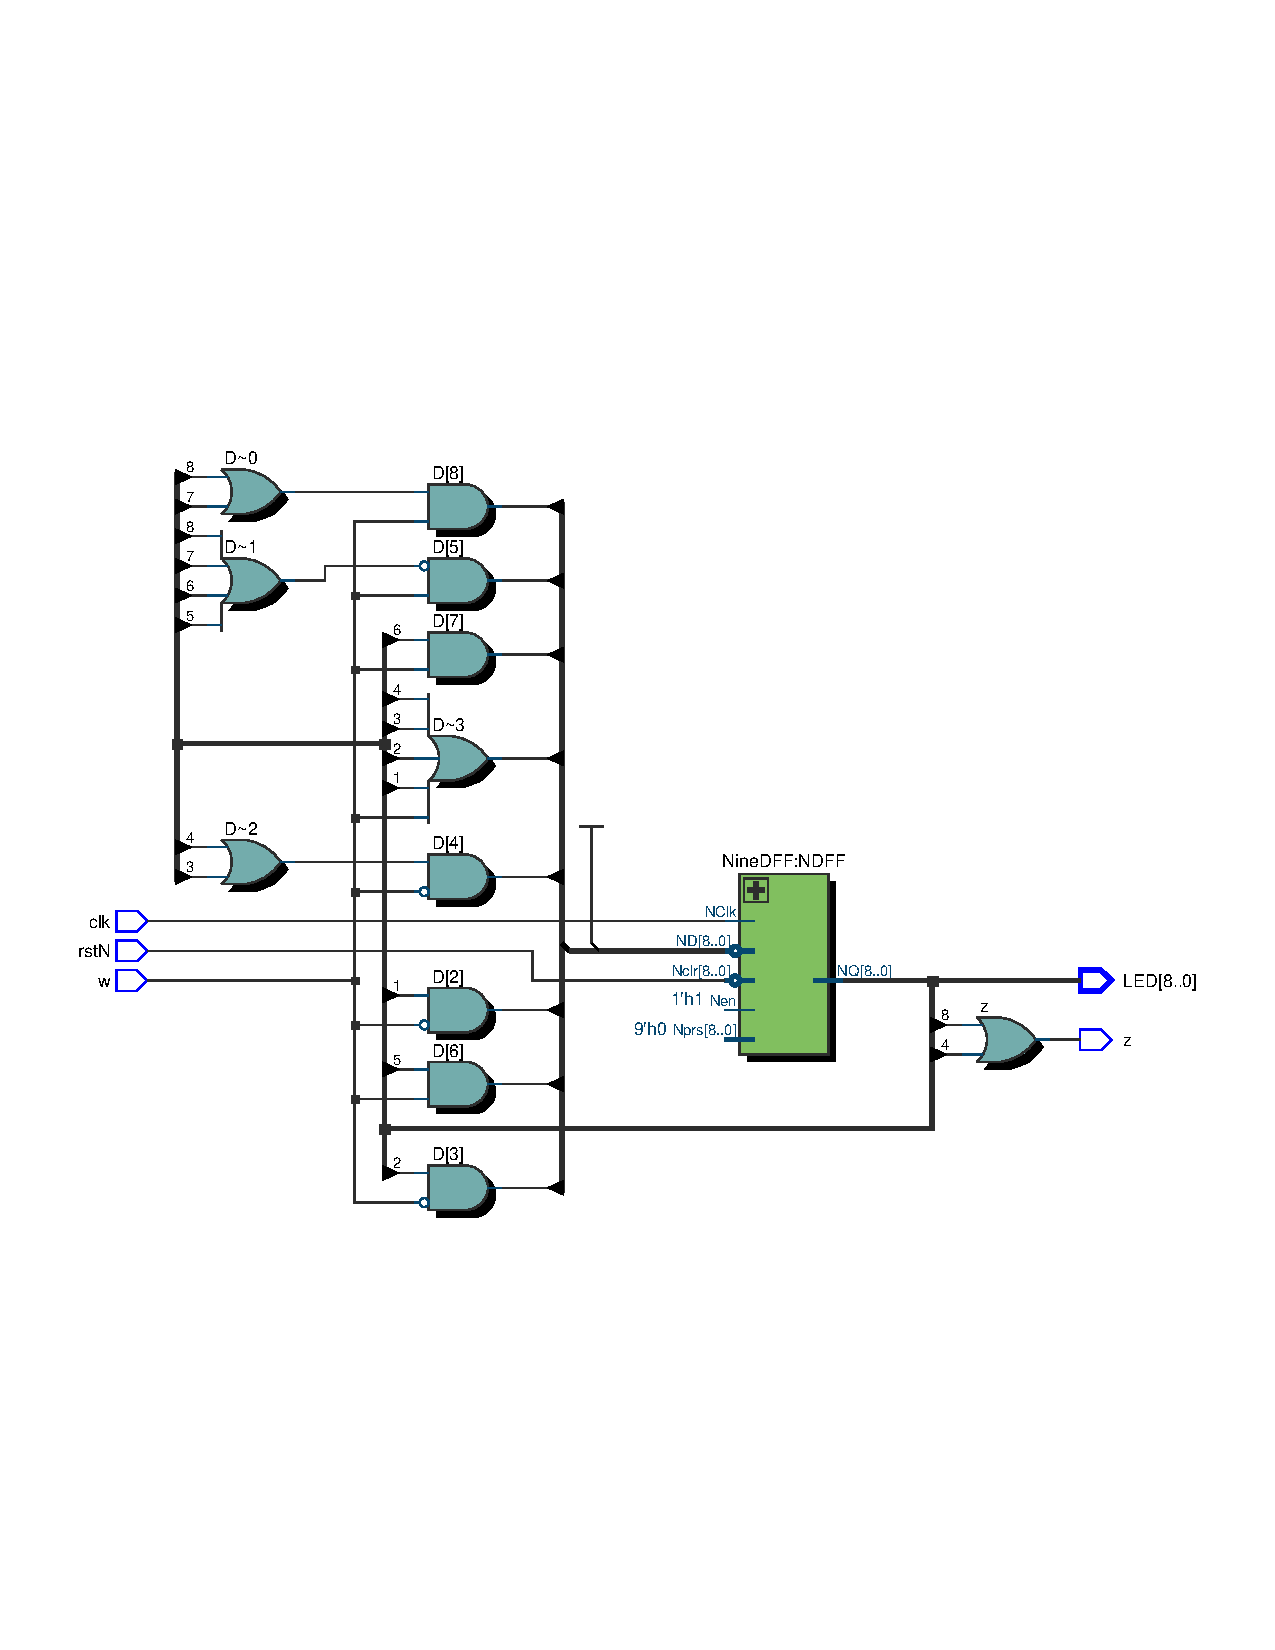
\includegraphics[scale=0.75, clip, trim={0cm 7cm 0cm 7.5cm}]{images/Exc1_RTL_2.pdf}
\caption*{Top level (using modified one-hot encoding)}
\end{figure}

\newpage
\section{Know how to implement a FSM circuit using VHDL behavioral expressions and download the cicuit into the FPGA chip}
\subsection{Code}
\subsubsection{Exc2.vhd}
\begin{minted}{vhdl}
LIBRARY ieee;
USE ieee.std_logic_1164.ALL;
ENTITY Exc2 IS PORT (
	w, clk, rst : IN STD_LOGIC;
	x : OUT STD_LOGIC
);
END Exc2;

ARCHITECTURE Behavior OF Exc2 IS
	TYPE State_type IS (A, B, C, D, E, F, G, H, I);
	ATTRIBUTE syn_encoding : STRING;
	ATTRIBUTE syn_encoding OF State_type : TYPE IS "0000 0001 0010 0011 0100 0101 0110 0111 1000";

	SIGNAL y_Q, Y_D : State_type;
BEGIN
	PROCESS (w, y_D)
	BEGIN
		CASE y_D IS
			WHEN A =>
				IF (w = '0') THEN 
					y_Q <= B;
				ELSE
					y_Q <= F;
				END IF;

			WHEN B =>
				IF (w = '0') THEN
					y_Q <= C;
				ELSE
					y_Q <= F;
				END IF;

			WHEN C =>
				IF (w = '0') THEN
					y_Q <= D;
				ELSE
					y_Q <= F;
				END IF;

			WHEN D =>
				IF (w = '0') THEN
					y_Q <= E;
				ELSE
					y_Q <= F;
				END IF;

			WHEN E =>
				IF (w = '0') THEN
					y_Q <= E;
				ELSE
					y_Q <= F;
				END IF;

				-------------------------
			WHEN F =>
				IF (w = '1') THEN
					y_Q <= G;
				ELSE
					y_Q <= B;
				END IF;

			WHEN G =>
				IF (w = '1') THEN
					y_Q <= H;
				ELSE
					y_Q <= B;
				END IF;

			WHEN H =>
				IF (w = '1') THEN
					y_Q <= I;
				ELSE
					y_Q <= B;
				END IF;

			WHEN I =>
				IF (w = '1') THEN
					y_Q <= I;
				ELSE
					y_Q <= B;
				END IF;
		END CASE;
	END PROCESS;
	x <= '1' WHEN y_D = E OR y_D = I ELSE '0';

	PROCESS (clk, rst)
	BEGIN
		IF rst = '1' THEN
			Y_D <= A;
		ELSE
			IF rising_edge(clk) THEN
				y_D <= y_Q;
			END IF;
		END IF;
	END PROCESS;
END Behavior;
\end{minted}

\subsection{Waveform}
\begin{figure}[H]
\centering
\includegraphics[scale=0.45]{images/Exc2_waveform.png}
\end{figure}

\subsection{Result of RTL viewer}
\begin{figure}[H]
\centering
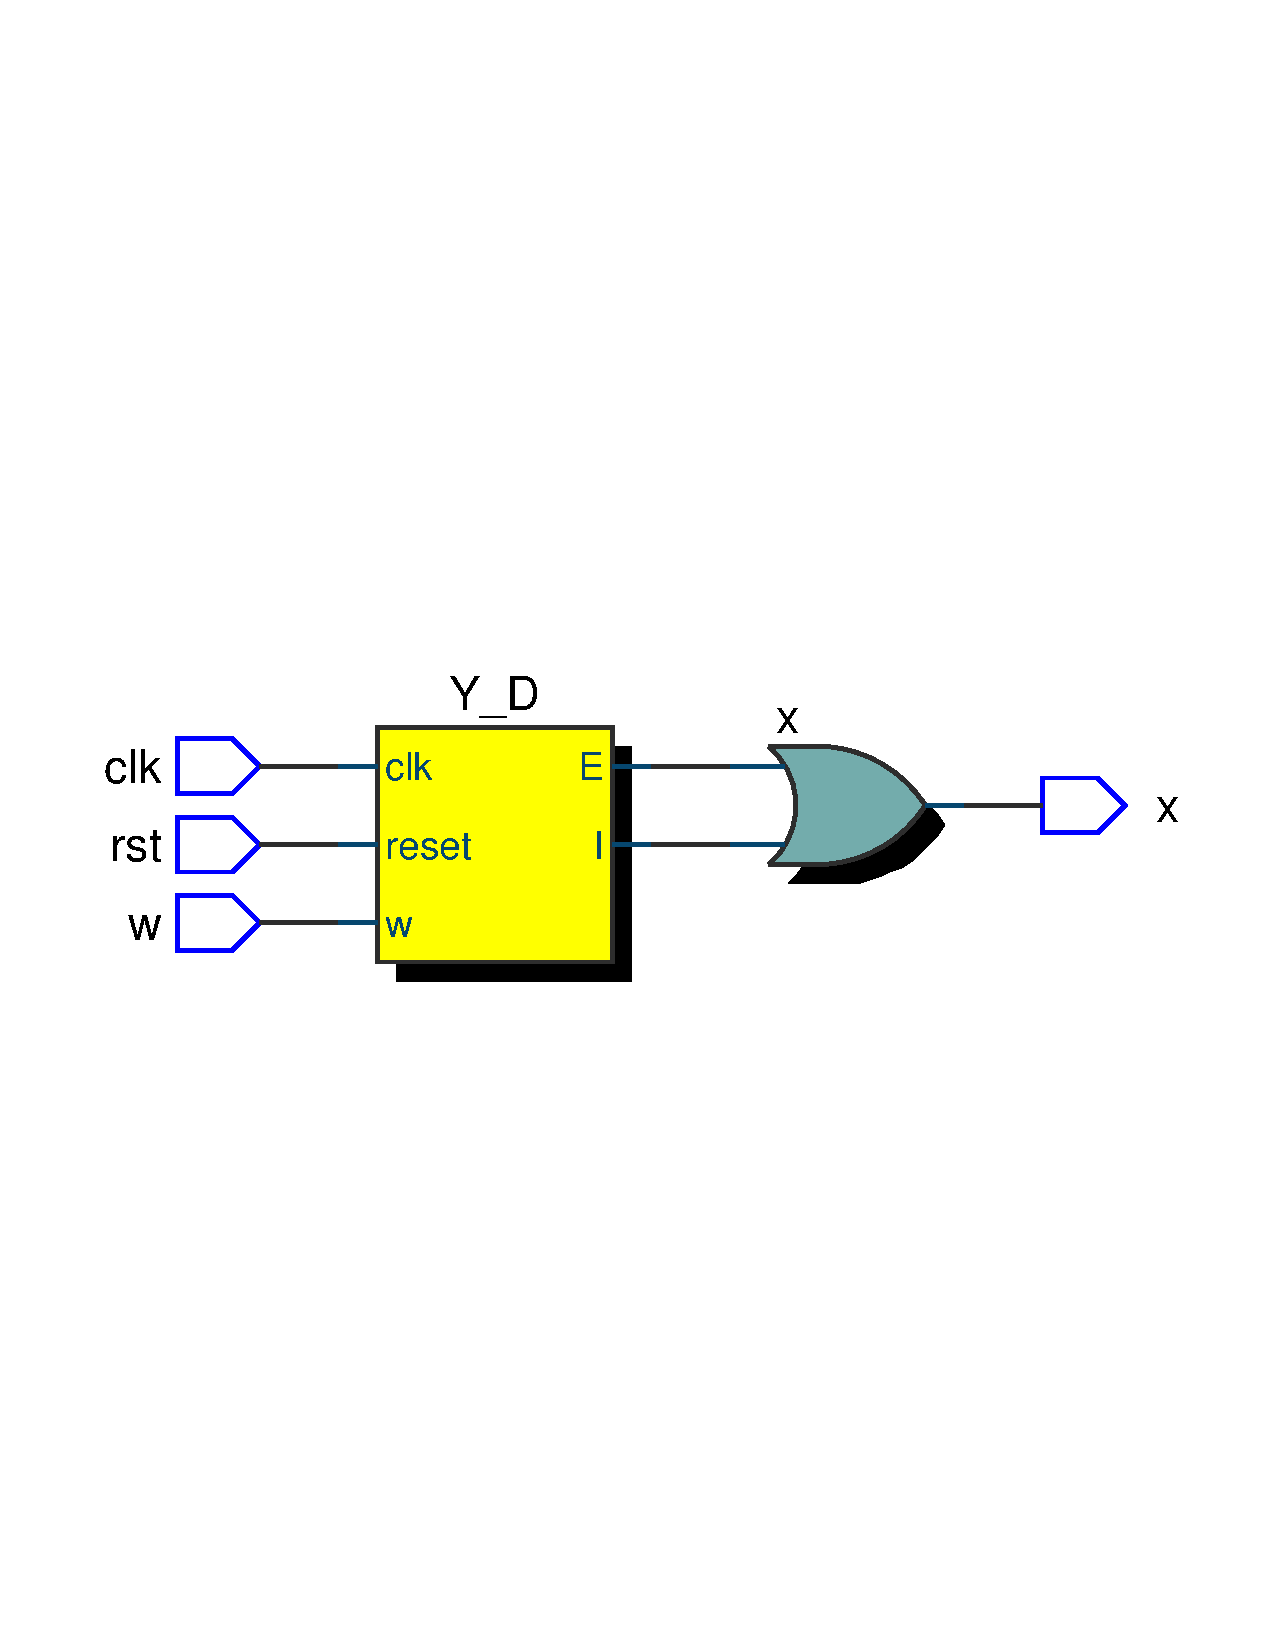
\includegraphics[scale=0.55, clip, trim={0cm 11cm 0cm 11cm}]{images/Exc2_RTL.pdf}
\caption*{Top level}
\end{figure}

\subsection{State machine diagram and encoding types}
\begin{figure}[H]
\centering
\includegraphics[scale=0.6, clip, trim={0cm 7.3cm 0cm 3.8cm}]{images/Exc2_FSM.pdf}
\caption*{State machine diagram}
\end{figure}

\begin{figure}[H]
\centering
\subfloat[][]{
\includegraphics[scale=0.6]{images/Exc2_encoding_1.png}
}
\subfloat[][]{
\includegraphics[scale=0.6]{images/Exc2_encoding_2.png}
}
\caption*{Encoding types}
\end{figure}

\newpage
\section{Know how to implement sequence detector using shift registers}

In this exercise, using two shift registers is a waste, so I will use only one shift register and connect it with some logic gates, that is enough.

\subsection{Code}
\subsubsection{DFFn.vhd}
\begin{minted}{vhdl}
LIBRARY ieee;
USE ieee.std_logic_1164.ALL;
ENTITY DFFn IS
	PORT (
		Din, DClk, DprsN, DclrN, Den : IN STD_LOGIC; -- clr and prs are active low.
		DQ : OUT STD_LOGIC);
END DFFn;
ARCHITECTURE Behavior OF DFFn IS
BEGIN
	PROCESS (DprsN, DclrN, DClk)
	BEGIN
		IF DclrN = '0' AND DprsN = '1' THEN
			DQ <= '0';
		ELSIF DclrN = '1' AND DprsN = '0' THEN
			DQ <= '1';
		ELSE
			IF rising_edge(DClk) AND Den = '1' THEN
				DQ <= Din;
			END IF;
		END IF;
	END PROCESS;
END Behavior;
\end{minted}

\subsubsection{FourBitShiftReg.vhd}
\begin{minted}{vhdl}
LIBRARY ieee;
USE ieee.std_logic_1164.ALL;
USE ieee.numeric_std.ALL;

ENTITY FourBitShiftReg IS
	PORT (
		SRegclk, SReginp, SRegrstN : IN STD_LOGIC;
		SRegL : OUT STD_LOGIC_VECTOR(0 TO 3)
	);
END FourBitShiftReg;

ARCHITECTURE arch OF FourBitShiftReg IS
	SIGNAL q : STD_LOGIC_VECTOR(0 TO 3) := "XXXX";
	COMPONENT DFFn IS
		PORT (
			Din, DClk, DprsN, DclrN, Den : IN STD_LOGIC;
			DQ : OUT STD_LOGIC);
	END COMPONENT;
BEGIN
	DFF0 : DFFn PORT MAP(
		Din => SReginp, DClk => SRegclk, DprsN => '1',
		DclrN => SRegrstN, Den => '1', DQ => q(0));
	gen : FOR i IN 1 TO 3 GENERATE
		DFFs : DFFn PORT MAP(
			Din => q(i - 1), DClk => SRegclk, DprsN => '1',
			DclrN => SRegrstN, Den => '1', DQ => q(i));
	END GENERATE;
	SRegL <= q;
END ARCHITECTURE;
\end{minted}

\subsubsection{Exc2.vhd}
\begin{minted}{vhdl}
LIBRARY ieee;
USE ieee.std_logic_1164.ALL;
USE ieee.numeric_std.ALL;

ENTITY Exc3 IS
	PORT (
		inp, clk, rstN : IN STD_LOGIC;
		z : OUT STD_LOGIC
	);
END Exc3;

ARCHITECTURE arch OF Exc3 IS
	SIGNAL L : STD_LOGIC_VECTOR(0 TO 3);
	SIGNAL waitFourClocks : UNSIGNED(2 DOWNTO 0) := "100";
	SIGNAL en : STD_LOGIC;
	COMPONENT FourBitShiftReg IS
		PORT (
			SRegclk, SReginp, SRegrstN : IN STD_LOGIC;
			SRegL : OUT STD_LOGIC_VECTOR(0 TO 3)
		);
	END COMPONENT;
BEGIN
	PROCESS (clk)
	BEGIN
		IF rstN = '0' THEN
			waitFourClocks <= "100";
		ELSIF rising_edge(clk) AND waitFourClocks /= 0 THEN
			waitFourClocks <= waitFourClocks - 1;
		END IF;
	END PROCESS;
	en <= '1' WHEN waitFourClocks = 0 ELSE '0';
	SR1 : FourBitShiftReg PORT MAP(SRegclk => clk, SReginp => inp, SRegrstN => rstN, SRegL => L);

	z <= '1' WHEN (L1 = "1111" OR L1 = "0000") AND en = '1' ELSE '0';
END ARCHITECTURE;
\end{minted}

\subsection{Waveform}
\begin{figure}[H]
\centering
\includegraphics[scale=0.53]{images/Exc3_waveform.png}
\end{figure}

\subsection{Result of RTL viewer}
\begin{figure}[H]
\centering
\subfloat[][D flip-flop]{
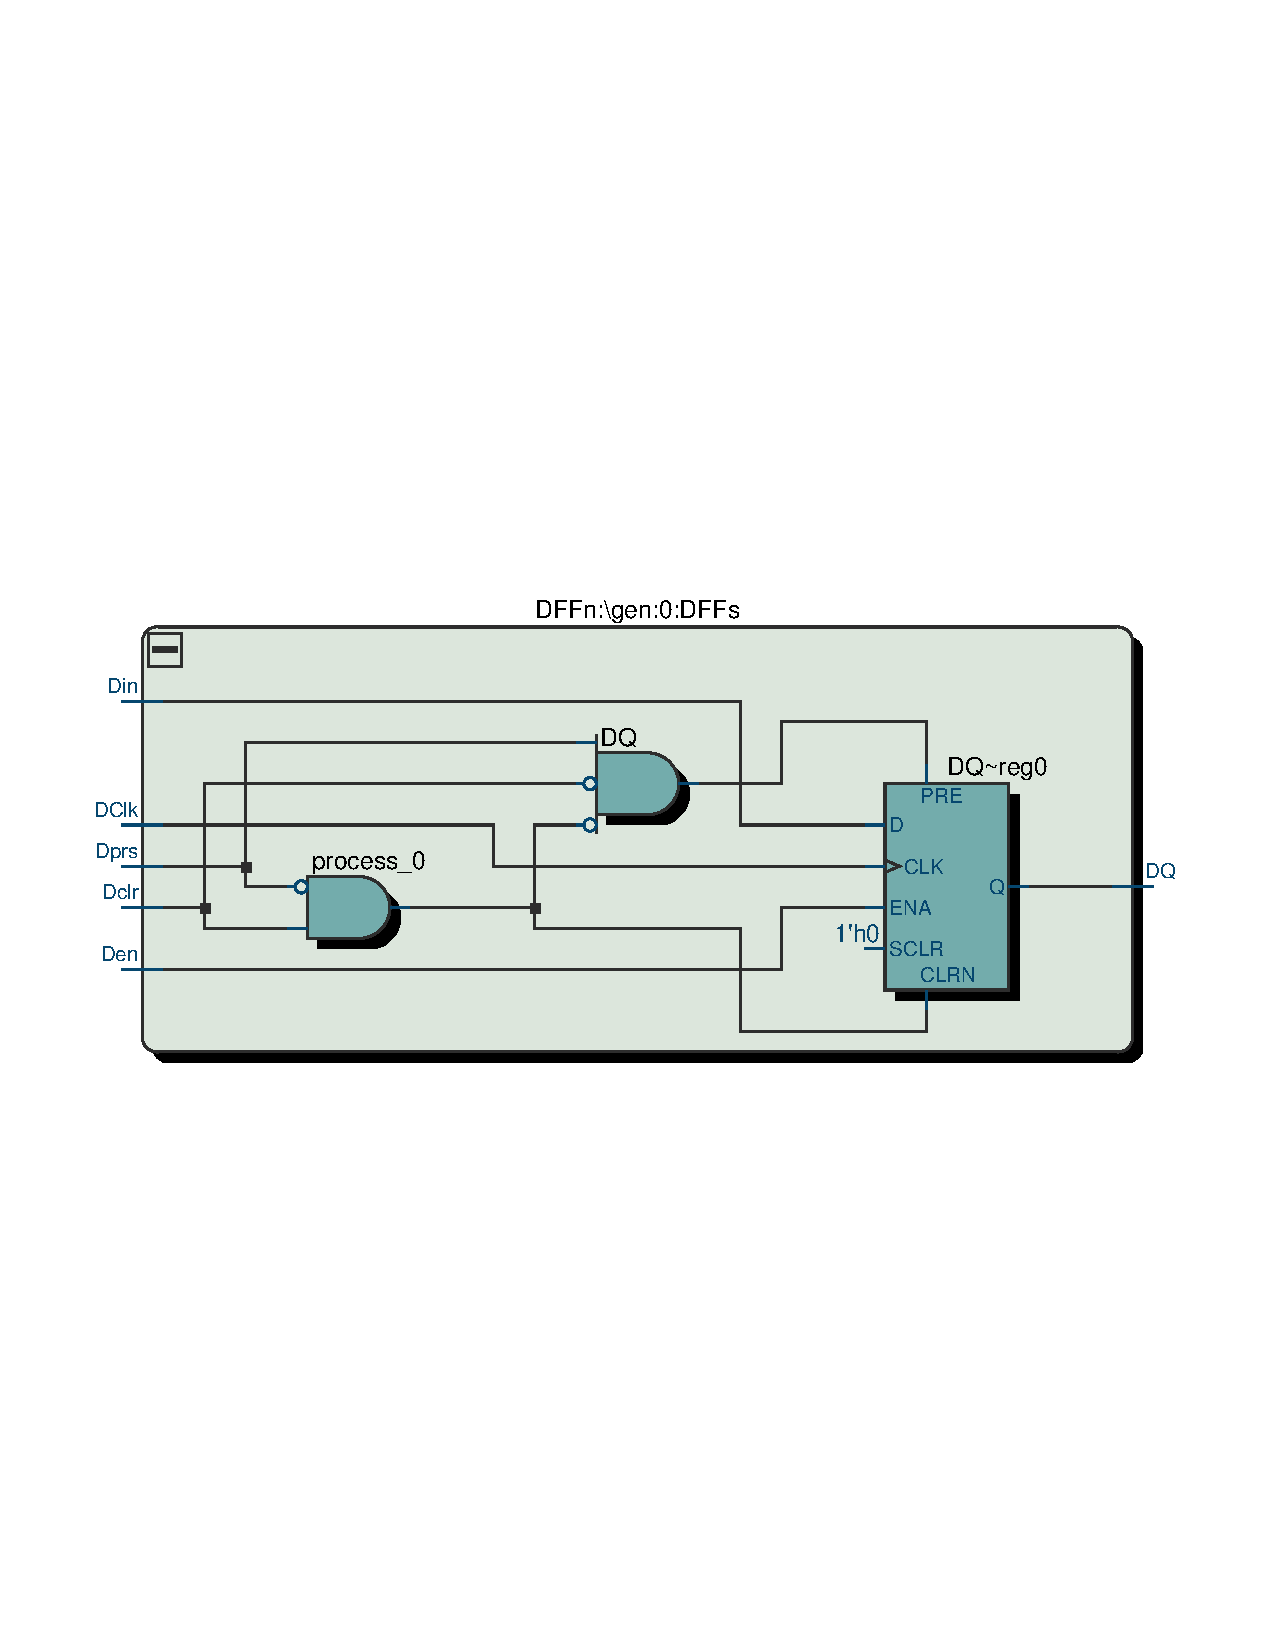
\includegraphics[scale=0.5, clip, trim={0cm 10cm 0cm 10.6cm}]{images/Exc1_DFF_RTL.pdf}
}
\subfloat[][Four-bit shift register]{
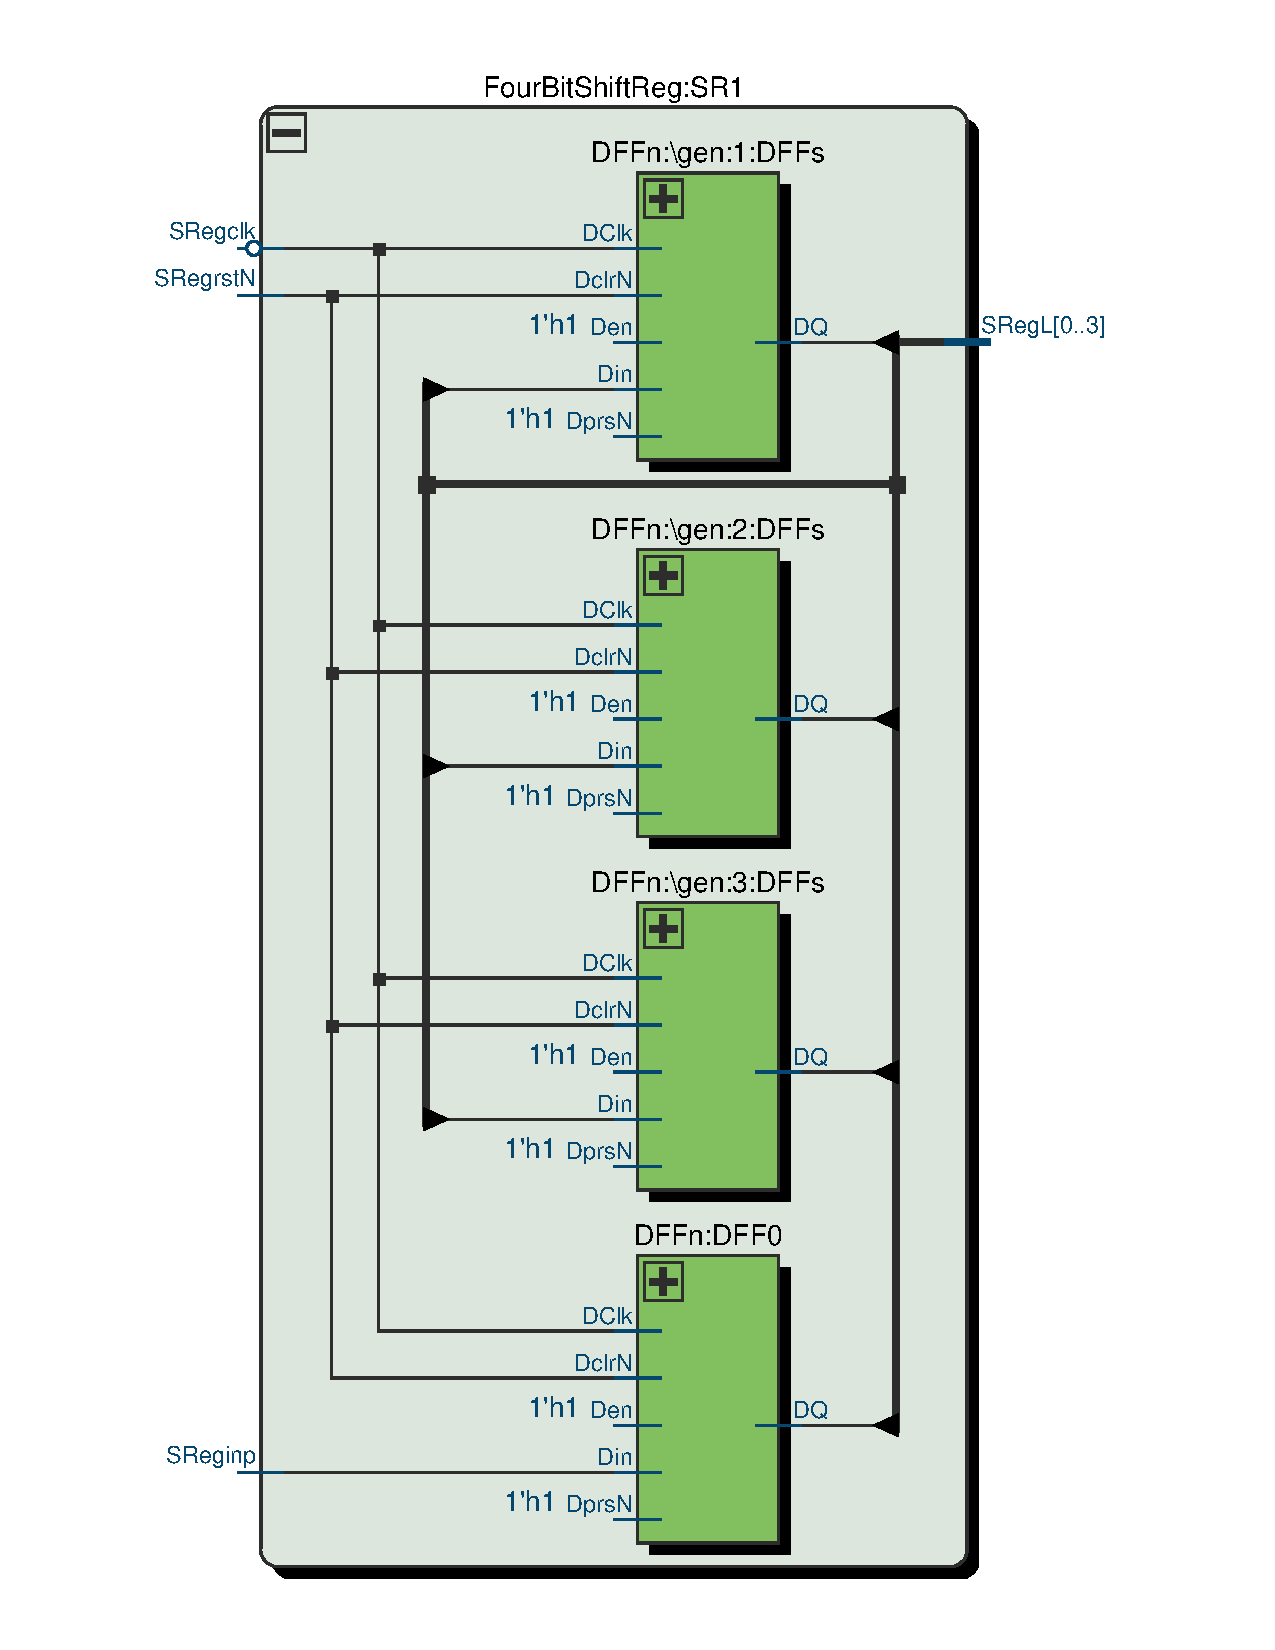
\includegraphics[scale=0.35, clip, trim={3cm 1cm 3cm 1.8cm}]{images/Exc3_FourBitShiftReg_RTL.pdf}
}
\end{figure}

\begin{figure}[H]
\centering
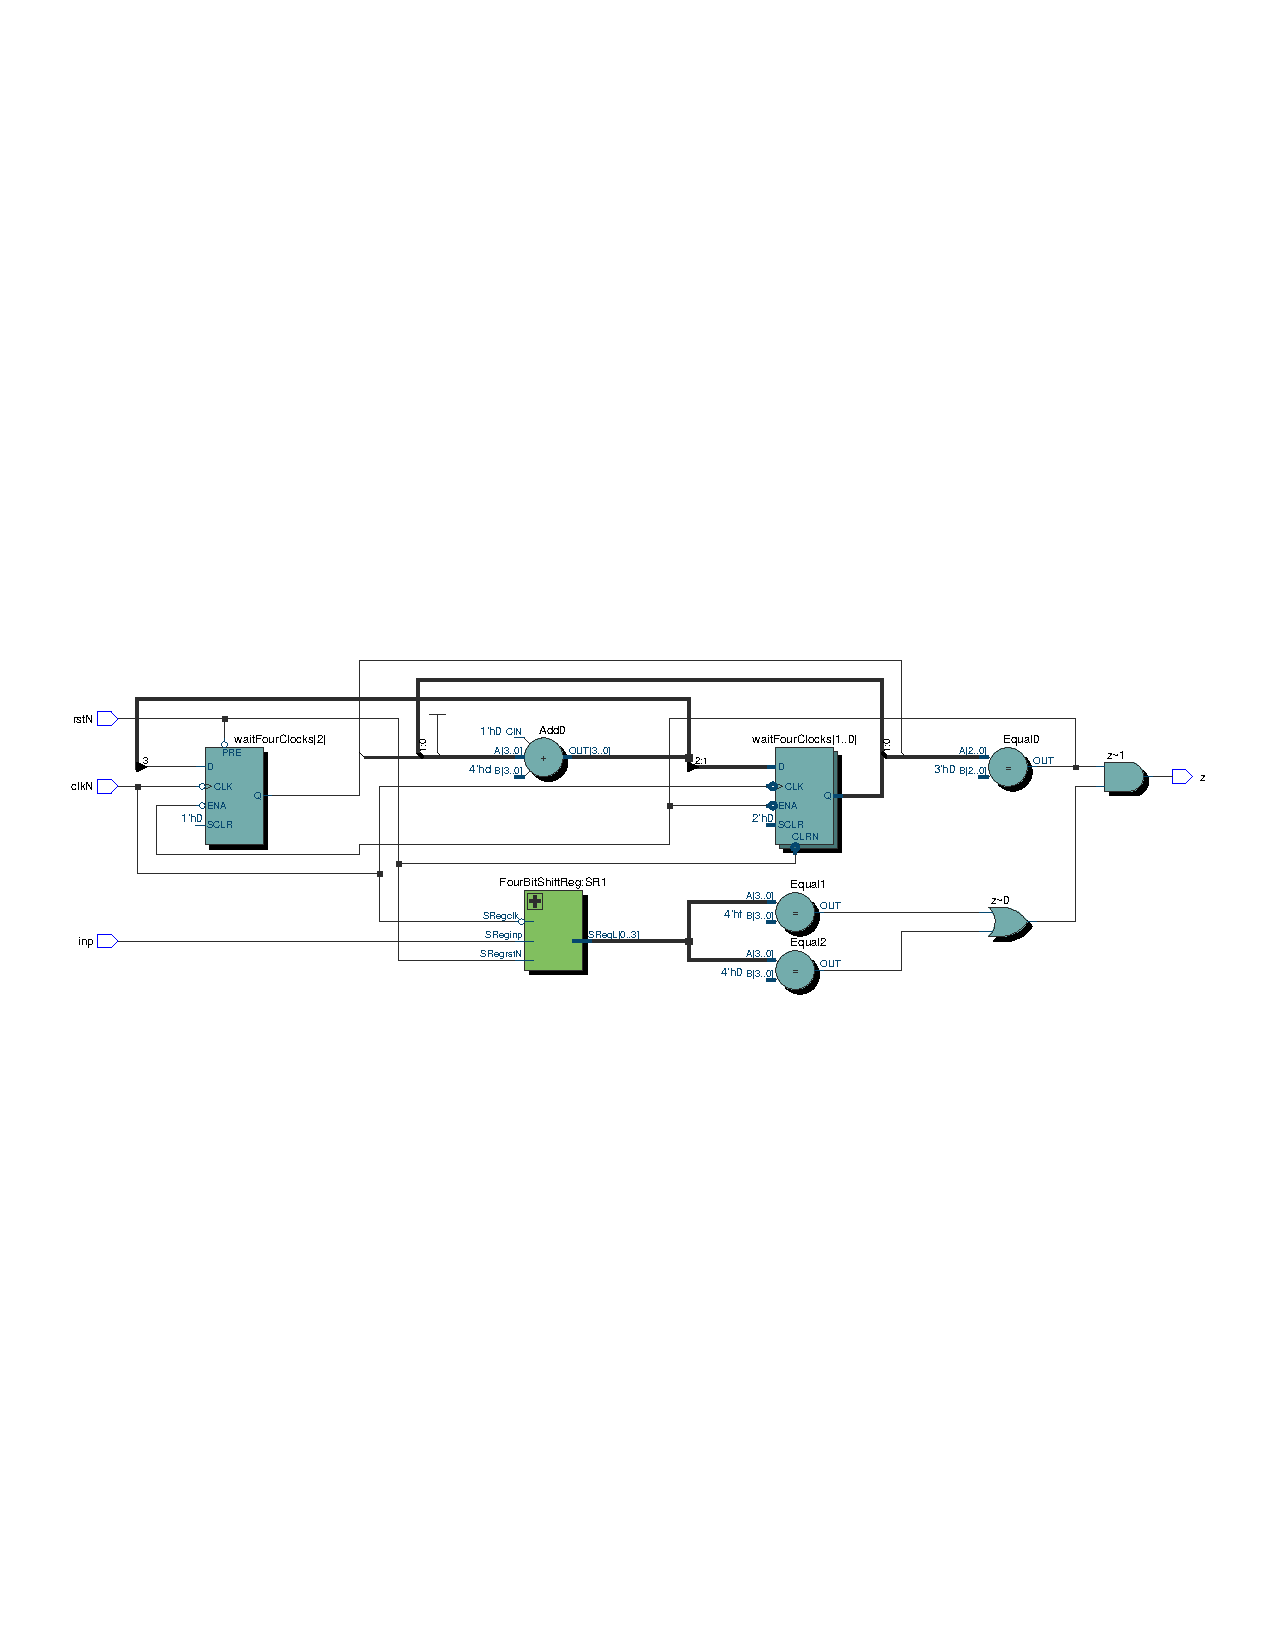
\includegraphics[scale=0.85, clip, trim={0cm 11cm 0cm 11cm}]{images/Exc3_RTL.pdf}
\caption*{Top level}
\end{figure}

\tikzset{
->, % makes the edges directed
>=stealth', % makes the arrow heads bold
node distance=5cm, % specifies the minimum distance between two nodes. Change if necessary.
every state/.style={thick, fill=gray!10}, % sets the properties for each ’state’ node
initial text=$ $, % sets the text that appears on the start arrow
}

\newpage
\section{Know how to implement a digital circuit using an FSM}
As I stated in PreLab 4, in this exercise, instead of using two LEDR and LEDG, I modifed the circuit, so when there is a dot, LED will on for 0.25 second; when there is a dash, LED will on for 1 second.

\subsection{FSM diagram}
\begin{figure}[H]
\centering
\scalebox{0.8}{
\begin{tikzpicture}
\node[state, initial] (idle) {idle};
\node[state, right of=idle] (store) {store};
\node[state, right of=store] (shift) {\makecell{Shift \&\\decrease size}};
\node[state, right of=shift] (setT) {\makecell{Set\\wait time}};
\node[state, below of=setT] (wait) {wait};
\node[state, left of=wait] (dec) {\makecell{Wait\\LED off}};
\node[state, left of=dec] (check) {\makecell{Check\\size}};

\draw (idle) edge[loop above] node{btn = 0} (idle)
(idle) edge[above] node{btn = 1} (store)
(store) edge[above] node{} (shift)
(shift) edge[above] node{shifted bit} (setT)
(setT) edge[right] node{ticksToWait} (wait)
(wait) edge[loop below] node{ticks $<$ ticksToWait} (wait)
(wait) edge[above] node{ticks = ticksToWait} (dec)
(dec) edge[above] node{} (check)
(check) edge[left] node{size $>$ 0} (shift)
(check) edge[left] node{size = 0} (idle)
;
\end{tikzpicture}
}
\end{figure}

\subsection{Code}
\subsubsection{Exc4.vhd}
\begin{minted}{vhdl}
LIBRARY ieee;
USE ieee.std_logic_1164.ALL;
USE ieee.numeric_std.ALL;

ENTITY Exc4 IS
  PORT (
    letter : IN STD_LOGIC_VECTOR(2 DOWNTO 0);
    LED : OUT STD_LOGIC;
    clk, btnN, rstN : IN STD_LOGIC
  );
END Exc4;

ARCHITECTURE arch OF Exc4 IS
  SIGNAL morseCode : STD_LOGIC_VECTOR(3 DOWNTO 0);
  SIGNAL morseLength : STD_LOGIC_VECTOR(2 DOWNTO 0);
  SIGNAL bitIn, btn, rst : STD_LOGIC := '0';

  SIGNAL ticks, ticksToWait : INTEGER RANGE 0 TO 200 := 0; -- Change 200 to 50000000 if running on DE10.

  TYPE State_type IS (idle, store, shift, setWaitInterval, waitT, waitLEDOff, checkSize);
  SIGNAL state : State_type := idle;
  COMPONENT DFFn IS
    PORT (
      Din, DClk, Den : IN STD_LOGIC;
      DQ : OUT STD_LOGIC);
  END COMPONENT;

BEGIN
  btn <= NOT(btnN);
  rst <= NOT(rstN);
  PROCESS (clk, rst) IS
  BEGIN
    IF rst = '1' THEN
      state <= idle;
    ELSE
      IF rising_edge(clk) THEN
        CASE state IS
          WHEN idle =>
            LED <= '0';
            IF btn = '1' THEN
              state <= store;
            ELSE
              state <= idle;
            END IF;

          WHEN store =>
            CASE letter IS
              WHEN "000" =>
                morseCode <= "0010";
                morseLength <= "010";
              WHEN "001" =>
                morseCode <= "0001";
                morseLength <= "100";
              WHEN "010" =>
                morseCode <= "0101";
                morseLength <= "100";
              WHEN "011" =>
                morseCode <= "0001";
                morseLength <= "011";
              WHEN "100" =>
                morseCode <= "0000";
                morseLength <= "001";
              WHEN "101" =>
                morseCode <= "0100";
                morseLength <= "100";
              WHEN "110" =>
                morseCode <= "0011";
                morseLength <= "011";
              WHEN "111" =>
                morseCode <= "0000";
                morseLength <= "100";
              WHEN OTHERS =>
                morseCode <= "0000";
                morseLength <= "000";
            END CASE;
            state <= shift;

          WHEN shift =>
            bitIn <= morseCode(0);
            morseCode <= '0' & morseCode(3 DOWNTO 1); -- Shift;
            morseLength <= STD_LOGIC_VECTOR(UNSIGNED(morseLength) - 1);
            state <= setWaitInterval;

          WHEN setWaitInterval =>
            -- clk at 200Hz
            -- ticksToWait = oldFreq / newFreq
            -- dot = 4Hz (0.25s), dash = 1Hz (1s)
            IF (bitIn = '0') THEN
              ticksToWait <= 50; -- On DE10: 50MHz / 4Hz = 12500000
            ELSE
              ticksToWait <= 200; -- On DE10: 50MHz / 1Hz = 50000000
            END IF;

            ticks <= 0; -- Reset ticks
            LED <= '1'; -- LED on
            state <= waitT;

          WHEN waitT =>
            IF ticks = ticksToWait - 1 THEN
              LED <= '0'; -- LED off
              ticks <= 0; -- Reset ticks
              state <= waitLEDOff;
              ticksToWait <= 100;
            ELSE
              ticks <= ticks + 1;
              state <= waitT;
            END IF;

          WHEN waitLEDOff =>
            IF ticks = ticksToWait - 1 THEN
              state <= checkSize;
              ticks <= 0; -- Reset ticks
            ELSE
              ticks <= ticks + 1;
              state <= waitLEDOff;
            END IF;

          WHEN checkSize =>
            IF morseLength = "000" THEN
              state <= idle;
            ELSE
              state <= shift;
            END IF;
        END CASE;
      END IF;
    END IF;
  END PROCESS;
END ARCHITECTURE;
\end{minted}

\subsubsection{Exc4\_tb.vhd}
\begin{minted}{vhdl}
LIBRARY ieee;
USE ieee.std_logic_1164.ALL;
USE ieee.numeric_std.ALL;

ENTITY Exc4_tb IS
END ENTITY;

ARCHITECTURE sim OF Exc4_tb IS
	-- We're slowing down the clock to speed up simulation time
	CONSTANT ClockFrequencyHz : INTEGER := 200; -- 200 Hz
	CONSTANT ClockPeriod : TIME := 1000 ms / ClockFrequencyHz;

	SIGNAL letter : STD_LOGIC_VECTOR(2 DOWNTO 0) := "000";
	SIGNAL LED : STD_LOGIC;
	SIGNAL clk : STD_LOGIC := '1';
	SIGNAL btnN : STD_LOGIC := '0';
	SIGNAL rstN : STD_LOGIC := '1';
BEGIN
	-- The Device Under Test (DUT)
	morse : ENTITY work.Exc4(arch)
		PORT MAP(
			letter => letter,
			LED => LED,
			clk => clk,
			btnN => btnN,
			rstN => rstN
		);
	-- Process for generating the clock
	Clk <= NOT Clk AFTER ClockPeriod / 2;
	PROCESS IS
	BEGIN
		WAIT UNTIL rising_edge(clk);
		btnN <= '0';
		WAIT UNTIL rising_edge(clk);
		btnN <= '1';
		WAIT FOR 5000 ms;
		letter <= STD_LOGIC_VECTOR(UNSIGNED(letter) + 1);
	END PROCESS;
END ARCHITECTURE;
\end{minted}

\subsection{Waveform}
\begin{figure}[H]
\centering
\includegraphics[scale=0.38]{images/Exc4_waveform.png}
\end{figure}

\subsection{Result of RTL viewer}
\begin{figure}[H]
\centering
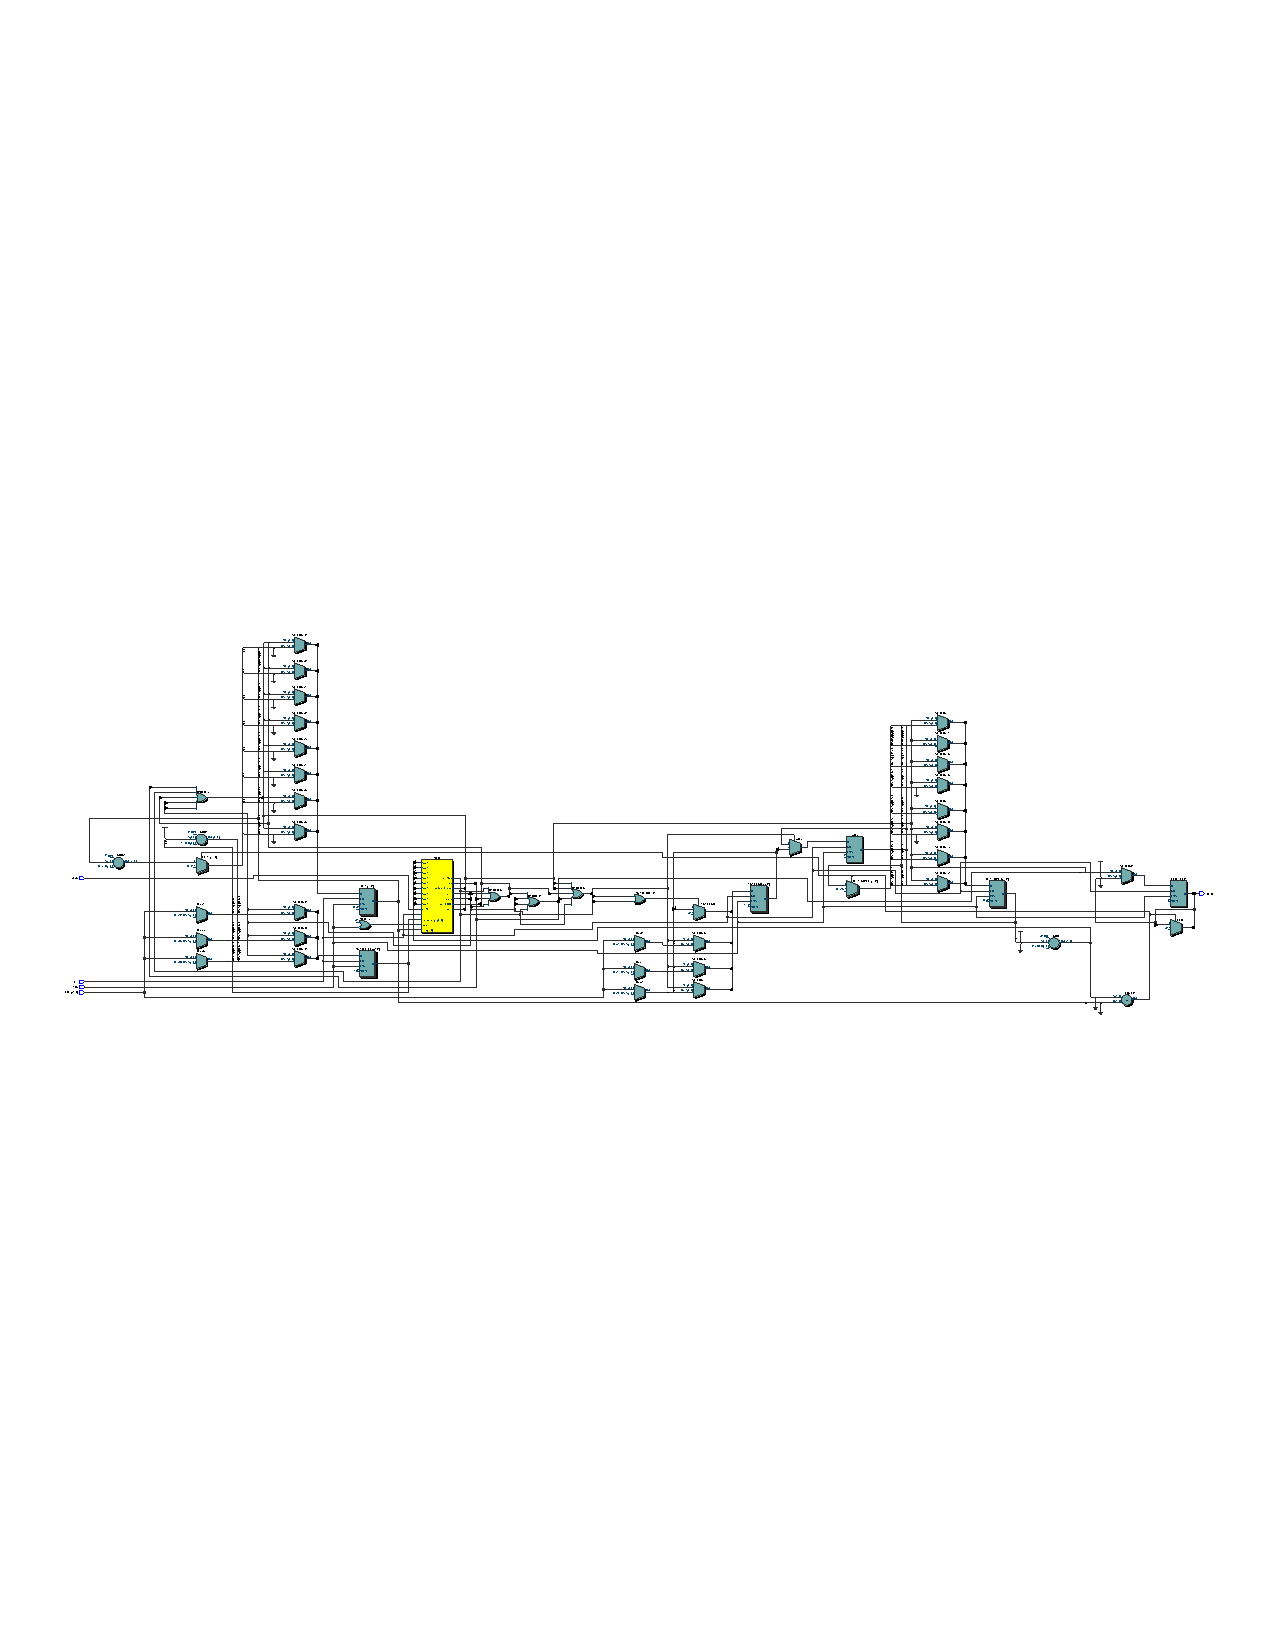
\includegraphics[scale=0.95, clip, trim={1cm 10.6cm 1cm 10.8cm}]{images/Exc4_RTL.pdf}
\caption*{Top level (zoom in for better viewing)}
\end{figure}

\subsection{State machine diagram}\begin{figure}[H]
\centering
\includegraphics[scale=0.8, clip, trim={5cm 7.3cm 3cm 5cm}]{images/Exc4_FSM.pdf}
\end{figure}
\end{document}